\documentclass[a4paper,12pt]{article}
\usepackage{url}
\usepackage{listings}
\usepackage{color}
\usepackage{hyperref}
\usepackage{graphicx}
\usepackage{booktabs}
%\usepackage{mdframed}
\usepackage{adjustbox}

\definecolor{dkgreen}{rgb}{0,0.6,0}
\definecolor{gray}{rgb}{0.5,0.5,0.5}
\definecolor{mauve}{rgb}{0.58,0,0.82}

\lstset{frame=tb,
	language=C++,
	aboveskip=3mm,
	belowskip=3mm,
	showstringspaces=false,
	columns=flexible,
	basicstyle={\small\ttfamily},
	numbers=none,
	numberstyle=\tiny\color{gray},
	keywordstyle=\color{blue},
	commentstyle=\color{dkgreen},
	stringstyle=\color{mauve},
	breaklines=true,
	breakatwhitespace=true,
	tabsize=3
}
\begin{document}
	
	\title{CS-224 Object Oriented Programming and Design Methodologies }
	\author{Homework 05}
	\date{Spring 2022}
	\maketitle
	\section{Guidelines}
	
	You need to submit this homework on  {\color{blue}08th April at 8pm}, on LMS. Late submissions are allowed until {\color{red} 10th April 11:59pm}, which will be penalized by 20\%. Your work will not be accepted once the submission is closed on LMS.

	
	\begin{itemize}
		\item You need to do this assignment in a group of two students.
		\item You will submit your assignment to LMS (only one member of the group will submit).
		\item Clearly mention the group composition in submitted file name e.g. AhmadHassan\_ah01345\_BatoolAiman\_ba03451.zip. 
		\item You need to follow the best programming practices 
		\item Submit assignment on time; late submissions will not be accepted.
		\item Some assignments will require you to submit multiple files. Always Zip and send them.
		\item It is better to submit incomplete assignment than none at all.
		\item It is better to submit the work that you have done yourself than what you have plagiarized.
		\item It is strongly advised that you start working on the assignment the day you get it. Assignments WILL take time.
%		\item Every assignment you submit should be a single zipped file containing all the other files. Suppose your name is John Doe and your id is 0022 so the name of the submitted file should be JohnDoe0022.zip
		\item DO NOT send your assignment to your instructor, if you do, your assignment will get ZERO for not following clear instructions.
		\item You can be called in for Viva for any assignment that you submit
	\end{itemize}
	
	
%\section{Bank Accounts}
%Please refer to HW4, where you already have solved this question. In this homework you need to draw UML diagram. Show all the classes, and put relevant attributes/functions in each class. Use appropriate arrows to show relationships among the classes. For a reference, the question is reproduced here.
%
%In this question you are going to develop a little simulation of banking accounts. You need to think in terms of objects encapsulated with attributes and their functions. 
%
%
%The first object is a \texttt{Bank} which have a \texttt{vector} of \texttt{Accounts}. Each Account object have certain balance and it can be manipulated with a \texttt{Deposit} and \texttt{Withdrawal} transactions. To maintain record, the \texttt{Account} need to store all the transactions executed on it, hence vectors of transactions can be part of an \texttt{Account} object. After executing all the transactions any account with less than 5000 available balance will become dormant, otherwise it is active. A \texttt{Date} class can be created that handles all tasks related to it.
%
%
%You need to model all the classes that can be found in this scenario e.g. \texttt{Bank, Account, Deposit, Withdraw, Date...}  You may create any other class/functions/attributes as deemed appropriate or necessary.
%
%\subsection*{Input File Processing}
%A sample input file is as follows:
%\begin{lstlisting}
%	Create Jasmin_Banda JB230 70000
%	Deposit GH090 30000 11-Mar
%	Withdrawal GH090 4000 12-April-21
%\end{lstlisting}
%Please refer to file \path{bankinput.txt} which contains certain entries to process. You can find three different types of entries in the file:
%\begin{itemize}
%	\item \texttt{Create Title Code InitialDeposit:} This entry creates an account with account title, code and initial deposit
%	\item \texttt{Deposit Code Amount Date:} This entry deposits the given amount in the particular account as per code. Date can vary in different forms, you have to adjust all of the forms e.g. default year is 2021, and it should accept all forms of the months.
%	\item \texttt{Withdrawal Code Amount Date:} This entry withdraws the amount from given account successfully if the available balance is sufficient to withdraw the money, else the transaction should fail. Date can vary in different forms, you have to adjust all of the forms e.g. default year is 2021, and it should accept all forms of the months.
%\end{itemize}
%
%\subsection*{Output File}
%After executing all the transactions from input file, your program should generate an output \path{bankoutput.txt} file, as per following sample it should print information of all accounts.
%\begin{lstlisting}
%	
%	Account Title: Saeed Ghani
%	Account Code: GH090
%	Initial Balance: 2000
%	Available Balance: 28000
%	Current Status: Active
%	Deposits: 
%	1. 30000 on 11/03/21
%	Withdrawals: 
%	1. 4000 on 12/04/21 Successful
%	2. 40000 on 15/06/21 Denied
%	
%\end{lstlisting}	

	

	\section{HUMania++}
	
	This is an extension to HUMania developed in HW4. Now you have to improve it by implementing inheritance, and showing polymorphism. 
	
	A sample code is given in HUMania folder, if you run it you can see a pigeon is drawn. This example creates just one object of Pigeon to show how things are drawn in SDL. Refer to \texttt{Pigeon.hpp/cpp and HUMania.cpp $ \Rightarrow $ drawObjects()}.
	
	 You are required to:
	 \begin{itemize}
	 	\item Create a class \texttt{Unit}, which deals with drawing of an object. It has a \texttt{draw} method, completely implemented, and it draws one of the three states of object. It also have \texttt{fly} method, since fly behavior is different for different types of objects, therefore it's not fully implemented rather it's made \texttt{virtual}.
	 	
	 	\item Create a \texttt{Pigeon} class inherited from \texttt{Unit}. It over-rides the \texttt{fly} function, that flies the pigeon gradually to right side, and rotates through the screen. 
	 	
	 	\item Create a \texttt{Butterfly} class inherited from \texttt{Unit}. It over-rides the \texttt{fly}function, that should take the butterfly right-down direction. Once a butterfly reaches to bottom of the screen, it starts flying right-up direction. Once it reaches top of the screen it moves right-down. Similar to the pigeon, it should rotate through the screen. 
	 	
	 	\item Create a \texttt{Bee} class inherited from \texttt{Unit}. It over-rides the fly function, that should make it fly towards right only. During fly it should hover (doesn't move forward) for a while over a random interval. You may choose 1\% probability in every frame to decide whether it starts hover, and it keeps hovering for 10 frames. As a bee reaches to right most border of screen, it exits from the game, hence the object must be removed from the bees vector.  
	 	
	 	\item Every object animates three of the images provided in the assets file. The draw function is only drawing the object.
	 	
	 	\item As you click on the screen, one of the above objects is created randomly. Let's create a class \texttt{ObjectCreator}, it has only one function \texttt{Unit* getObject()}. This function creates one of the objects (Pigeon, Butterfly, Bee) randomly, and returns the pointer to that object. You'll maintain just a single list of \texttt{Unit*} to store objects of all the types. Simply iterate over the list and call draw and fly functions of each object. 
	 	
	 	\item You have to create objects dynamically with \texttt{new} operator, hence the list should hold pointers to all of the objects. Remember to delete the objects when game is ended, and when the bee objects are removed from vector.
	 	
	 	\item As you are maintaining a single list to store all types of objects, therefore it would be essential to find out the Bee objects, because it's required to remove Bee objects when they leave the window. For this task you have to identify the type of objects. Please \href{https://en.cppreference.com/w/cpp/language/typeid}{refer to this page} to find type.
	 	
%	 	\item Finally, you iterate over all the elements of vectors, and call their fly and draw functions.
	 	
	 	\item Please refer to \path{Solution.exe} file to see it all in action.
	 	
%	 	\item You also have to draw a UML diagram for this question.
	 	
	 	\item Are you having fun?? You are more than welcome to add more stuff to make this game interesting, e.g. some natural random movement of butterflies, sitting them on ground, pigeons sweeping etc. [\textit{It doesn't carry any marks}]
	 \end{itemize}
 

%	\begin{figure}
%		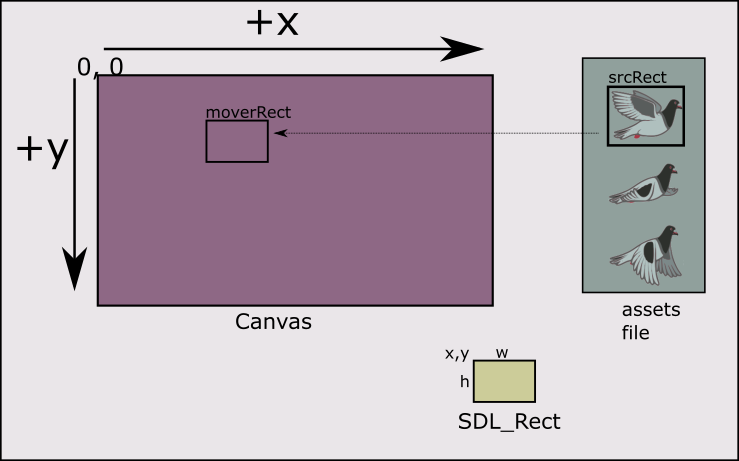
\includegraphics[width=\linewidth]{sdlDrawing}
%		\caption{SDL Drawing Basics}
%		\label{fig:sdlDrawing}
%	\end{figure}  

	
	
%	\subsection{SDL Drawing Basics}
%	
%	The basic drawing function in SDL is very simple, you need two SDL\_Rect variables to draw a portion of image from assets file to the canvas. \texttt{SDL\_Rect} is a simple structure containing \texttt{\{x, y, w, h\} }attributes. \texttt{(x, y)} is the top-left corner, and \texttt{w, h} are width and height of rectangle. You define a \texttt{srcRect} for desired object in assets file, and define a \texttt{moverRect} for this image to be drawn on desired location on canvas. Refer to Figure \ref{fig:sdlDrawing} for all this process.  Finally you call 
%	
%	\noindent \texttt{SDL\_RenderCopy(gRenderer, assets, \&pigeonSrc, \&pigeonMover);}
%	
%	\noindent that displays this image to the canvas, voila!!!. Refer to \texttt{assets.png} file for all the required image assets.
%	
%	You can draw as many objects in the \texttt{HUMania.cpp $ \Rightarrow $ drawObjects()}, as you want. Since this function is called infinitely, you can change the \texttt{x, y} attributes of \texttt{moverRect} to move the objects on screen, and you can change the \texttt{srcRect} values to get a flying animation.
%	

\pagebreak

\section{\texttt{std::list} Tutorial} \label{vectorTutorial}

list is an std library's doubly linked list implementation. It provides constant time insertion and deletion operations, but it doesn't support indexing. You can look for complete manual here: \url{https://en.cppreference.com/w/cpp/container/list}.

\begin{lstlisting}
#include<iostream>
#include<list>

using namespace std;

class Distance{
	int feet, inches;
	public:
	Distance(int ft, int inch): feet(ft), inches(inch){}
	void show(){
		cout<<feet<<"'"<<inches<<"\""<<endl;
	}
};

int main(){
	list<Distance*> dst; // It's a list that can store Distance type objects
	dst.push_back(new Distance(3, 4)); // create an object, and push it in vector
	dst.push_back(new Distance(5, 2));
	dst.push_back(new Distance(2, 7));
	dst.push_back(new Distance(7, 8));
	dst.push_back(new Distance(13, 1));
	
	for(Distance* d: dst){	// list doesn't support indexing, but we can use python's style for loop.
		d->show(); 			
	}
	
	// deleting the objects, need to delete every single object created dynamically
	for(Distance* d: dst){
		delete d;
	}
	
	dst.clear(); //clears all the items from vector
	
}
//////////////// Output: ///////////////////
3'4"
5'2"
2'7"
7'8"
13'1"
\end{lstlisting}


\section{Some important points:} 

\begin{itemize}
	\item Sample code is there for your benefit. If you are going to use it, understand how it works. 
	\item You do not need to follow the code given exactly. You can make changes where you see fit provided that it makes sense.
	\item Make the class declarations in hpp files, and provide function implementations in cpp files. Don't use hpp files for implementation purposes.
	\item \href{https://www.techiedelight.com/remove-elements-vector-inside-loop-cpp/}{A tutorial given here} to remove the elements from vector, you might need it to remove bees as they exit the screen.
	%		\item Implement Q1 prior to implementing Q2, it will help you to implement linked list.
	%		\item Where necessary, declare your own functions inside classes. Make sure why you would keep a function as private or public.
	\item As a general rule, class's deta is private, and functions are public. Don't use getter/setter functions to manipulate data, rather think in object oriented directions and provide all the functionality in the class.
	\item Complete reference for C++ list is given here \url{https://en.cppreference.com/w/cpp/container/list}
	\item You need to define separate \path{*.hpp} and \path{*.cpp} files for all the classes.
	\item Exact x,y,w,h values for images in assets file can be found by \url{http://www.spritecow.com/}. 
	\item A tutorial for file I/O is given \url{http://www.cplusplus.com/doc/tutorial/files/}. 
	\item You should take \url{www.cplusplus.com} and \url{www.cppreference.com} as primary web source to search about C++
%	\item You can choose any tool of your choice to draw UML diagrams, however \url{draw.io} is a good online tool.
	\item You have to follow best OOP practices as discussed in lectures.
\end{itemize}

\section{How to compile}
Open the given \texttt{HUMania} folder in vscode by choosing \texttt{File $\Rightarrow$ Open Folder}. The game can be run by simply pressing F5 from vscode. If due to some reason it doesn't work, then go compiling and running it from terminal, as explained in \texttt{how to compile.txt}


\section{Rubric}
\begin{table}[!h]
	\centering
	\begin{tabular}{llc}
		\toprule
%		Warnings/Errors	& The code had no warnings/errors/	& 1 \\
%		Comments &	The code was properly commented	& 1 \\
%		Coding	& UML diagram is drawn for both questions &	5 \\
		OOP Concepts & Inheritance and polymorphism is well implemented & 5 \\
		 Memory &	Dynamic memory management is done properly	& 3\\
		Functionality	& All the functionality is implemented as described above	& 2 \\
		\midrule
		Total & & 10\\
		\bottomrule
	\end{tabular}
	\caption{Grading Rubric}
	\label{Grading}
\end{table}


	
	
\end{document}